\documentclass{beamer}
\usetheme{Madrid}

\title[Wobbling Motion in Odd-Mass Nuclei] % (optional, only for long titles)
{Wobbling Motion in odd-mass nuclei}
\author[R. Poenaru] % (optional, for multiple authors)
{Robert Poenaru\inst{1,2}}
\institute[DFT @ IFIN-HH] % (optional)
{
  \inst{1}%
  Department of Theoretical Physics\newline
  IFIN-HH
  \and
  \inst{2}%
  Faculty of Physics\newline
  University of Bucharest
}
\date[\today] % (optional)
{Bucharest University Faculty of Physics 2021 Meeting}
\subject{Nuclear Physics}

\begin{document}
\maketitle
\begin{frame}
\frametitle{Table of Contents}
\tableofcontents
\end{frame}

\section{Triaxial nuclei}

\begin{frame}{Triaxiality}
\begin{itemize}
    \item Nuclear shapes: most of the nuclei are spherical or axially symmetric in the ground state.
    \item There are also deviations from \emph{axial symmetric shapes} $\to$ \textbf{triaxial shapes} (e.g. no symmetry axis).
\end{itemize}
  \begin{figure}
    \centering
    % \includegraphics[scale=0.65]{figs/prolate.pdf}
    \caption{\textbf{Spherical:} $\beta_2=0$ ; \textbf{Prolate:} $\beta_2>0$ ; \textbf{Oblate:} $\beta_2<0$}
  \end{figure}
\end{frame}

\begin{frame}{Nuclear deformation}
    \begin{block}{Nuclear surface - axially-symmetric shape}
    \begin{itemize}
    \item The shape of the nucleus can be described via the \textit{deformation parameters} $\beta,\gamma$. 
    \item They arise from the shape parameterization of the nuclear surface.
    \begin{align}
        R(\theta,\phi)=R_0\left(1+\sum_{\lambda=2}^{\infty}\sum_{\mu=0}^{\lambda}\alpha_{\lambda\mu}Y_{\lambda\mu}(\theta,\phi)\right)
    \end{align}
    \item For axial-quadrupole deformed nuclei $\beta_2=\alpha_{20}$.
    \end{itemize}
    \end{block}
\end{frame}

\begin{frame}{Deformation parameters}
    \begin{block}{Nuclear surface - axially-asymmetric shape}
    \begin{itemize}
    \item For nuclei with the three principal axes of different lengths (\emph{axial asymmetry}), the $\gamma$ deformation parameter emerges.
    \item Relationship between $\beta,\gamma$ and the expansion coefficients from the expression of $R(\theta,\phi)$ is given by:
    \begin{align}
        \alpha_{20}&=\beta_2\cos\gamma\\
        \alpha_{22}&=\frac{1}{\sqrt{2}}\beta_2\sin\gamma
    \end{align}
    \end{itemize}
    \end{block}
\end{frame}

\begin{frame}{Nuclear Wobbling Motion}
      \begin{figure}
          \centering
          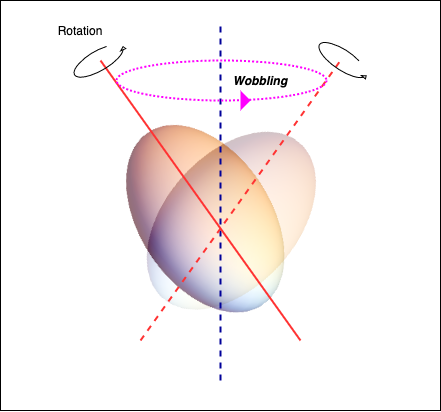
\includegraphics[scale=0.45]{figs/wobbling_drawing.png}
          \caption{Schematic representation for the nuclear wobbling motion.}
          \label{wobbling_picture}
      \end{figure}
\end{frame}



\section{Results}  

\begin{frame}
    \frametitle{Example of columns 1}
    \begin{columns}[c] % the "c" option specifies center vertical alignment
    \column{.45\textwidth} % column designated by a command
     Contents of the first column
    \column{.45\textwidth}
     Contents split \newline into two lines
    \end{columns}
\end{frame}

\section{Conclusions}

  \begin{frame}
  \centering
    \Large{Thank you for your attention!}
  \end{frame}

\end{document}